\documentclass[11pt,a4paper]{article}

% === Packages ===
\usepackage[utf8]{inputenc}
\usepackage[T1]{fontenc}
\usepackage{amsmath,amssymb,amsthm}
\usepackage{enumitem}
\usepackage{hyperref}
\usepackage{cleveref}
\usepackage{tikz}
\usepackage{tikz-cd}
\usepackage{booktabs}
\usepackage{geometry}
\usepackage{xcolor}
\usepackage{tcolorbox}
\usepackage{fancyvrb}
\usepackage{listings}

\geometry{margin=1in}
\hypersetup{colorlinks=true,linkcolor=blue!70!black,citecolor=green!50!black,urlcolor=purple!70!black}

% === Theorem environments ===
\theoremstyle{plain}
\newtheorem{theorem}{Theorem}[section]
\newtheorem{proposition}[theorem]{Proposition}
\newtheorem{lemma}[theorem]{Lemma}
\newtheorem{corollary}[theorem]{Corollary}

\theoremstyle{definition}
\newtheorem{definition}[theorem]{Definition}
\newtheorem{example}[theorem]{Example}
\newtheorem{remark}[theorem]{Remark}

% === Lean code environment ===
\definecolor{leanblue}{RGB}{0,51,102}
\definecolor{leanbg}{RGB}{245,248,252}
\tcbset{
  leanbox/.style={colback=leanbg, colframe=leanblue!60,
    fonttitle=\bfseries\ttfamily, title=#1,
    boxrule=0.5pt, arc=2pt, left=4pt, right=4pt}
}

\definecolor{codegreen}{rgb}{0,0.6,0}
\definecolor{codegray}{rgb}{0.5,0.5,0.5}
\definecolor{codepurple}{rgb}{0.58,0,0.82}
\definecolor{backcolour}{rgb}{0.95,0.95,0.92}

\lstdefinestyle{leanstyle}{
  backgroundcolor=\color{backcolour},
  commentstyle=\color{codegreen},
  keywordstyle=\color{blue},
  stringstyle=\color{codepurple},
  basicstyle=\ttfamily\footnotesize,
  breaklines=true,
  keepspaces=true,
  numbers=left,
  numberstyle=\tiny\color{codegray},
  showstringspaces=false,
  tabsize=2,
  frame=single,
  escapeinside={(*@}{@*)},
  morekeywords={theorem,def,axiom,inductive,structure,where,instance,
    namespace,end,open,import,noncomputable,deriving,by,exact,intro,
    apply,simp,ring,norm_num,native_decide,decide,rfl,sorry,have,let,
    if,then,else,match,with,fun,forall,exists,Prop,Type,
    Classical,choice,propext,Quot,constructor,refine}
}

% === Macros ===
\newcommand{\BISH}{\textsf{BISH}}
\newcommand{\WKL}{\textsf{WKL}}
\newcommand{\DC}{\textsf{DC}}
\newcommand{\WLPO}{\textsf{WLPO}}
\newcommand{\LLPO}{\textsf{LLPO}}
\newcommand{\LPO}{\textsf{LPO}}
\newcommand{\MP}{\textsf{MP}}
\newcommand{\CLASS}{\textsf{CLASS}}
\newcommand{\CRM}{\textsf{CRM}}
\newcommand{\Z}{\mathbb{Z}}
\newcommand{\Q}{\mathbb{Q}}
\newcommand{\R}{\mathbb{R}}
\newcommand{\C}{\mathbb{C}}
\newcommand{\F}{\mathbb{F}}
\newcommand{\N}{\mathbb{N}}
\newcommand{\PP}{\mathbb{P}}
\DeclareMathOperator{\tr}{tr}
\DeclareMathOperator{\ord}{ord}
\DeclareMathOperator{\Spec}{Spec}
\DeclareMathOperator{\Hom}{Hom}
\DeclareMathOperator{\Aut}{Aut}
\DeclareMathOperator{\End}{End}
\DeclareMathOperator{\GL}{GL}
\DeclareMathOperator{\SL}{SL}
\DeclareMathOperator{\Gal}{Gal}
\DeclareMathOperator{\DR}{DR}
\DeclareMathOperator{\Sol}{Sol}
\DeclareMathOperator{\IndCoh}{IndCoh}
\DeclareMathOperator{\QCoh}{QCoh}
\DeclareMathOperator{\Loc}{Loc}
\renewcommand{\Re}{\operatorname{Re}}

% === Title ===
\title{\textbf{CRM Audit of the Riemann-Hilbert Correspondence:\\
Constructive Cost of the Regular Holonomic Equivalence\\
via the Gauss Hypergeometric Equation}\\[6pt]
\large Paper 106 of the Constructive Reverse Mathematics Series\\[6pt]
\normalsize\textit{Eighteenth CRMLint Application}}

\author{Paul Chun-Kit Lee\\
\small New York University, Brooklyn, New York\\
\small\texttt{dr.paul.c.lee@gmail.com}}
\date{March 2026}

\begin{document}
\maketitle

\begin{abstract}
We execute the first Constructive Reverse Mathematics (\CRM) audit of the regular holonomic Riemann-Hilbert (RH) correspondence, decomposing the proof of Deligne (1970), Kashiwara (1984), and Mebkhout (1980) into 16 atomic components across four phases.
The decomposition yields $10\ \BISH + 4\ \WLPO + 1\ \LPO + 1\ \CLASS = 16$ classified components (62.5\% constructive).
Three theorems emerge:
(A)~Deligne's canonical extension --- the quasi-inverse of the RH functor --- is constructively equivalent to \LPO{} via the spectral partition $0 \le \Re(\lambda) < 1$;
(B)~GAGA (G\'eom\'etrie Alg\'ebrique et G\'eom\'etrie Analytique) descent is the \emph{unique} \CLASS{} component: Cartan's Theorems~A/B via Montel's theorem (sequential compactness), confirming the Archimedean Obstruction Thesis (AOT; Paper~98);
(C)~for rational parameters, the Deligne obstruction collapses to \BISH, witnessed by the test case ${}_2F_1(\tfrac{1}{4}, \tfrac{1}{3}; \tfrac{2}{3}; z)$ on $\PP^1 \setminus \{0,1,\infty\}$.
The Lean~4 formalization (404 lines, 0~\texttt{sorry}) verifies the algebraic content via \texttt{norm\_num}/\texttt{decide} and documents the logical boundaries with typed axioms.
\end{abstract}

% ============================================================
\section{Introduction}
% ============================================================

The Riemann-Hilbert correspondence is among the deepest structural results in complex algebraic geometry: it establishes a categorical equivalence between regular holonomic $\mathcal{D}$-modules on a smooth complex variety $X$ and constructible sheaves of $\C$-vector spaces on $X^{\mathrm{an}}$.
In its strongest form (Kashiwara \cite{Kashiwara1984}, Mebkhout \cite{Mebkhout1980}), it extends Deligne's classical work on regular singular connections \cite{Deligne1970} to the derived category.

From the standpoint of Constructive Reverse Mathematics, the RH correspondence is a natural target for logical cost analysis.
It sits at the interface between algebraic and analytic geometry --- precisely the fault line identified by the Archimedean Obstruction Thesis (Paper~98, Theorem~5.1).
The algebraic de~Rham side operates over discrete polynomial rings; the Betti side requires evaluation of transcendental period integrals.
The correspondence functor must bridge this gap.

\subsection{Main results}

\begin{theorem}[Theorem A --- Deligne's Canonical Extension $\Leftrightarrow$ \LPO]
The quasi-inverse of the regular RH correspondence requires \LPO.
Specifically, Deligne's canonical extension (Proposition~II.5.4 of \cite{Deligne1970}) forces a spectral partition $0 \le \Re(\lambda) < 1$ on eigenvalues of the local monodromy logarithm, which is constructively equivalent to the floor function $\lfloor \cdot \rfloor : \R \to \Z$.
By Bridges--Richman \cite{BridgesRichman1987}, the floor function is equivalent to \LPO.
For rational parameters ($\lambda \in \Q$), the floor function is \BISH-computable.
\end{theorem}

\begin{theorem}[Theorem B --- Archimedean Obstruction Thesis Validation]
GAGA descent (Component~16) is the \emph{unique} \CLASS{} component of the RH correspondence.
The proof relies on Cartan's Theorems~A and~B: finite-dimensionality of coherent sheaf cohomology on compact analytic spaces, established via Montel's theorem (sequential compactness in spaces of holomorphic functions).
Montel's theorem is irreducibly non-constructive.
The connection coefficients (Kummer matrices), despite being transcendental Gamma-function ratios, are \BISH-computable: $\Gamma$ at non-integral rational arguments admits explicit Cauchy sequences with constructive moduli of convergence (the functional equation $\Gamma(s) = \Gamma(s{+}1)/s$ reduces negative fractional arguments to the strictly positive domain).
The sole \CLASS{} obstruction passes through infinite-dimensional topology, not through transcendental evaluation, confirming Paper~98, Theorem~5.1.
\end{theorem}

\begin{theorem}[Theorem C --- Rational Collapse]
For the Gauss hypergeometric equation ${}_2F_1(a,b;c;z)$ with $a,b,c \in \Q$ and all exponent differences non-integral, the Deligne canonical extension is \BISH: the spectral partition reduces to integer floor on rationals.
The algebraic de~Rham complex, indicial roots, exponent differences, non-resonance conditions, and Fuchs relation are all verified by \texttt{norm\_num} in Lean~4.
\end{theorem}

\subsection{\CRM{} primer}

We work in Bishop's constructive mathematics (\BISH) as the base system.
The hierarchy of omniscience principles used in this paper is:
\[
\BISH \subset \BISH + \WLPO \subset \BISH + \LPO \subset \CLASS.
\]
\WLPO{} (Weak Limited Principle of Omniscience) asserts that every binary sequence is all zeros or not all zeros.
\LPO{} (Limited Principle of Omniscience) asserts that every binary sequence has a 1 or is all zeros.
\CLASS{} denotes full classical logic (Law of Excluded Middle).
See Paper~1 of the series \cite{Paper1} for full definitions.

\subsection{State of the art}

The logical content of the Riemann-Hilbert correspondence has not previously been analyzed from a constructive standpoint.
Classical proofs follow Deligne \cite{Deligne1970} for the ODE case (regular singular connections on curves), extended to higher dimensions by Kashiwara \cite{Kashiwara1984} and independently by Mebkhout \cite{Mebkhout1980}.
The irregular case was resolved by D'Agnolo--Kashiwara \cite{DAgnoloKashiwara2016}, which we flag as future work (the Stokes phenomena introduce additional constructive obstructions).

Katz \cite{Katz1970} gave an algebraic criterion for regular singularity.
Beukers and Heckman \cite{BeukersHeckman1989} computed monodromy groups for hypergeometric equations.
None of these works address the constructive status of their arguments.

\subsection{Atlas fit}

This paper extends the CRMLint pipeline (Paper~76) to the interface between algebraic and analytic geometry.
It complements the Gauss-Manin squeeze (Paper~80), the differential Galois squeeze (Paper~82), and the Archimedean Obstruction Thesis (Paper~98).
The test case ${}_2F_1(\tfrac{1}{4}, \tfrac{1}{3}; \tfrac{2}{3}; z)$ reuses the Picard-Fuchs infrastructure of Papers~80--84.

% ============================================================
\section{Preliminaries}
% ============================================================

\begin{definition}[Regular singular connection]
Let $X$ be a smooth algebraic variety over $\C$ and $\mathcal{M}$ a coherent $\mathcal{D}_X$-module.
We say $\mathcal{M}$ is \emph{regular holonomic} if it is holonomic (characteristic variety purely of dimension $\dim X$) and has regular singularities in the sense of Katz--Oda \cite{Katz1970}: at each singular point, formal solutions have at most polynomial growth.
\end{definition}

\begin{definition}[Constructible sheaf]
A sheaf $\mathcal{F}$ of $\C$-vector spaces on $X^{\mathrm{an}}$ is \emph{constructible} if there exists a stratification $X = \bigsqcup S_i$ by locally closed algebraic subvarieties such that $\mathcal{F}|_{S_i}$ is a local system of finite rank for each $i$.
\end{definition}

\begin{definition}[The Riemann-Hilbert functors]
The de~Rham functor $\DR : D^b_{\mathrm{rh}}(\mathcal{D}_X) \to D^b_c(X^{\mathrm{an}}, \C)$ sends $\mathcal{M} \mapsto \Omega^\bullet_X \otimes^L_{\mathcal{D}_X} \mathcal{M}$.
The solution functor $\Sol : D^b_{\mathrm{rh}}(\mathcal{D}_X)^{\mathrm{op}} \to D^b_c(X^{\mathrm{an}}, \C)$ sends $\mathcal{M} \mapsto R\mathcal{H}om_{\mathcal{D}_X}(\mathcal{M}, \mathcal{O}_{X^{\mathrm{an}}})$.
Kashiwara's theorem: $\DR$ is an equivalence of triangulated categories.
\end{definition}

\begin{definition}[Deligne's canonical extension]
Let $\rho : \pi_1(U) \to \GL_n(\C)$ be a monodromy representation on $U = X \setminus D$ where $D$ is a normal crossing divisor.
Deligne constructs a unique algebraic vector bundle $\overline{\mathcal{E}}$ on $X$ with logarithmic connection $\nabla : \overline{\mathcal{E}} \to \overline{\mathcal{E}} \otimes \Omega^1_X(\log D)$ whose monodromy is $\rho$, by choosing the matrix logarithm $E_i = \frac{1}{2\pi i} \log T_i$ with eigenvalues satisfying $0 \le \Re(\lambda) < 1$ at each component of $D$.
\end{definition}

\begin{definition}[Omniscience principles {\cite{BridgesRichman1987}}]\label{def:omniscience}
\LPO: $\forall \alpha : \N \to \{0,1\}$, either $\exists n.\, \alpha(n) = 1$ or $\forall n.\, \alpha(n) = 0$.\\
\WLPO: $\forall \alpha : \N \to \{0,1\}$, either $\forall n.\, \alpha(n) = 0$ or $\lnot(\forall n.\, \alpha(n) = 0)$.\\
Floor function: $\lfloor x \rfloor$ for $x \in \R$ is the unique $n \in \Z$ with $n \le x < n+1$.
Bridges--Richman: $\lfloor \cdot \rfloor$ exists for all $x \in \R$ if and only if \LPO{} holds.
\end{definition}

% ============================================================
\section{The 16-Component Decomposition}
% ============================================================

We decompose the proof of the regular holonomic RH correspondence into sixteen atomic components, grouped into four phases.
\Cref{tab:decomposition} summarizes the classification.

\begin{table}[ht]
\centering
\caption{CRM decomposition of the regular holonomic RH correspondence.}
\label{tab:decomposition}
\small
\begin{tabular}{clcl}
\toprule
\# & Component & Level & Obstruction \\
\midrule
\multicolumn{4}{c}{\textit{Phase A: Algebraic $\mathcal{D}$-Module Theory}} \\
1 & Weyl algebra \& differential operators & \BISH & Ring theory \\
2 & Holonomicity via characteristic variety & \BISH & Gr\"obner basis (Castro--Oaku) \\
3 & Katz algebraic regularity criterion & \BISH & Pole order bounds \\
4 & Algebraic de Rham complex & \BISH & Discrete tensor products \\
\midrule
\multicolumn{4}{c}{\textit{Phase B: Local Analytic Theory}} \\
5 & Frobenius formal solutions & \BISH & Decidable recurrence \\
6 & Cauchy majorant convergence & \BISH & Constructive error bounds \\
7 & Resonance decidability & \WLPO & $\lambda_1 - \lambda_2 = n$: equality test on $\C$ \\
8 & Identity theorem for germs & \WLPO & All Taylor coefficients vanish? \\
\midrule
\multicolumn{4}{c}{\textit{Phase C: Global Topological Theory}} \\
9 & Fundamental group presentation & \BISH & Zariski--van Kampen \\
10 & Picard-Lindel\"of continuation & \BISH & Constructive ODE theory \\
11 & Homotopy invariance of lifting & \WLPO & Identity theorem for germs \\
12 & Connection coefficient evaluation & \BISH & Computable $\Gamma$-ratios at $\Q$-arguments \\
13 & Constructibility of solution sheaf & \WLPO & Zero-testing of $\C$-determinants \\
\midrule
\multicolumn{4}{c}{\textit{Phase D: Equivalence Functors}} \\
14 & Analytification $\DR^{\mathrm{an}}$ & \BISH & Algebraic sheaf extension \\
15 & Deligne canonical extension & \LPO & Floor function $=$ \LPO \\
16 & GAGA descent & \CLASS & Cartan A/B via Montel (compactness) \\
\bottomrule
\end{tabular}
\end{table}

\subsection{Phase A: Algebraic $\mathcal{D}$-module theory (4 \BISH)}

Components 1--4 operate entirely over polynomial rings and their localizations.
The Weyl algebra $A_n(\C) = \C\langle x_1, \ldots, x_n, \partial_1, \ldots, \partial_n \rangle / ([\partial_i, x_j] = \delta_{ij},\, [x_i, x_j] = 0,\, [\partial_i, \partial_j] = 0)$ is a finitely presented non-commutative ring whose multiplication is algorithmically computable.
Holonomicity is decidable via the algorithms of Castro-Jim\'enez \cite{Castro1987} and Oaku \cite{Oaku1997}: computing the dimension of the characteristic variety reduces to a Gr\"obner basis computation in a polynomial ring, which is \BISH.
Katz's regularity criterion \cite{Katz1970} tests nilpotency of residue matrices and boundedness of pole orders --- again, finite linear algebra over the coefficient field.
The algebraic de~Rham complex $\Omega^\bullet_X \otimes_{\mathcal{O}_X} \mathcal{M}$ involves finite tensor products of finitely generated modules.

No archimedean limits appear.
These components validate the \emph{algebraic side} of the Archimedean Obstruction Thesis.

\subsection{Phase B: Local analytic theory (2 \BISH{} + 2 \WLPO)}

The Frobenius method (Component~5) extracts formal power series solutions $y(z) = z^\rho \sum a_n z^n$ from the indicial equation and a linear recurrence on the $a_n$.
For algebraic coefficients, this recurrence is decidable (\BISH).
Cauchy's method of majorants (Component~6) proves convergence by dominating the formal solution by a geometric series with explicit polynomial error bounds --- constructively valid following Bishop--Bridges \cite{BishopBridges1985}.

Component~7 (resonance) is the first non-trivial obstruction.
Two indicial roots $\rho_1, \rho_2$ are \emph{resonant} if $\rho_1 - \rho_2 \in \Z$.
For $\rho_i \in \Q$, this is a decidable integer test (\BISH).
For arbitrary $\rho_i \in \C$, testing $\rho_1 - \rho_2 = n$ for a candidate $n \in \Z$ is an equality test on $\C$.
The nearest integer candidate is constructively approximable (\BISH), so the obstruction reduces to deciding $z = 0$ for $z \in \C$, which is \WLPO.

Component~8 (identity theorem) states that if two holomorphic germs $f, g$ agree on an accumulation set, then $f = g$.
Constructively, this reduces to: given the Taylor coefficients $(a_n - b_n)_{n \ge 0}$, decide whether all are zero.
This is precisely \WLPO.

\subsection{Phase C: Global topological theory (3 \BISH{} + 2 \WLPO)}

The fundamental group $\pi_1(\PP^1 \setminus \{0,1,\infty\})$ has the finite presentation $\langle \gamma_0, \gamma_1, \gamma_\infty \mid \gamma_0 \gamma_1 \gamma_\infty = 1 \rangle$ by Zariski--van Kampen (\BISH).
Analytic continuation along a fixed compact path bounded away from singular points is constructive by Picard-Lindel\"of theory with explicit Lipschitz bounds (\BISH).

Homotopy invariance (Component~11) requires the identity theorem for germs along deformed paths, inheriting the \WLPO{} tag from Component~8.

Component~12 (connection coefficients) is \BISH, not \CLASS{} as one might naively expect.
The Kummer matrices bridge local solution bases at distinct singular points.
For ${}_2F_1(a,b;c;z)$, their entries are ratios of Gamma-function values at rational arguments:
\[
C_{01}[0,0] = \frac{\Gamma(c)\,\Gamma(c-a-b)}{\Gamma(c-a)\,\Gamma(c-b)}.
\]
These entries are transcendental but \emph{computable}: the Gamma function $\Gamma(s) = \int_0^\infty t^{s-1} e^{-t}\,dt$ at non-integral rational $s$ admits explicit geometric majorants and constructive moduli of convergence (Bishop--Bridges \cite{BishopBridges1985}).
The functional equation $\Gamma(s) = \Gamma(s{+}1)/s$ reduces negative fractional arguments (such as $\Gamma(-1/12)$) to the strictly positive domain.
Completing a computable Cauchy sequence of rationals is the \emph{definition} of a real number in \BISH, not a classical obstruction.
The Kummer ratios, being quotients of constructive reals with constructively provable non-vanishing denominators ($\Gamma(s) > 0$ for $s > 0$), are themselves \BISH-computable.

Constructibility (Component~13) requires proving that solution sheaf stalks are finite-dimensional.
Computing exact matrix ranks over $\C$ reduces to deciding whether complex-valued minors vanish: $\det(M) = 0$ or $\det(M) \neq 0$.
This is \WLPO{} (equality testing on $\C$), not \LPO{} (which would require real trichotomy).

\subsection{Phase D: Equivalence functors (1 \BISH{} + 1 \LPO{} + 1 \CLASS)}

The analytification functor (Component~14) extends algebraic sheaves to the analytic topology.
This is a formal operation that preserves the existing constructive content (\BISH).

Component~15 is the central theorem of this paper: Deligne's canonical extension.
See \Cref{sec:deligne} for the full analysis.

Component~16 (GAGA descent) requires Serre's theorem that coherent analytic sheaves on projective varieties are algebraic \cite{Serre1956}.
The \CLASS{} cost is Cartan's Theorems~A and~B: finite-dimensionality of coherent sheaf cohomology on compact analytic spaces, proved via Montel's theorem (compactness in spaces of holomorphic functions).
Montel's theorem is irreducibly non-constructive: it extracts convergent subsequences from bounded families using sequential compactness on $\C$.

% ============================================================
\section{The Sharpest Obstruction: Deligne's Canonical Extension}
\label{sec:deligne}
% ============================================================

\begin{theorem}[Theorem A, precise form]\label{thm:deligne-lpo}
Let $T \in \GL_n(\C)$ be a monodromy operator.
The existence of a matrix logarithm $E = \frac{1}{2\pi i} \log T$ with all eigenvalues $\lambda$ satisfying $0 \le \Re(\lambda) < 1$ is constructively equivalent to $\LPO$.
\end{theorem}

\begin{proof}
Given an eigenvalue $\lambda$ of $\frac{1}{2\pi i} \log T$ (which is determined up to integer shifts), Deligne's prescription requires computing $\lambda - \lfloor \Re(\lambda) \rfloor$ to shift $\lambda$ into the fundamental strip $[0,1)$.
This requires the floor function $\lfloor \cdot \rfloor : \R \to \Z$.

By Bridges and Richman \cite{BridgesRichman1987}, Chapter~6, Theorem~6.1:
the floor function is constructively equivalent to the Limited Principle of Omniscience.
Specifically, given $x \in \R$, to compute $\lfloor x \rfloor$ one must decide for each $n \in \Z$ whether $n \le x < n+1$.
This requires trichotomy on $\R$ (given $x, y \in \R$, decide $x < y$, $x = y$, or $x > y$), which is equivalent to \LPO.

Conversely, given \LPO, the floor function is computable: for each $n$, test $n \le x < n+1$ using the decidable order on $\R$ that \LPO{} provides.

For the special case $T$ with eigenvalues $e^{2\pi i \rho}$ where $\rho \in \Q$, the eigenvalue $\rho$ of the logarithm is rational, and $\lfloor \rho \rfloor$ is decidable by integer arithmetic.
Thus the canonical extension is \BISH{} for rational exponents.
\end{proof}

\begin{remark}
The \LPO{} cost of the Deligne extension is \emph{sharper} (more precisely localizable) than the \CLASS{} cost of GAGA descent, even though the latter is logically \emph{stronger}.
In CRM auditing, sharpness means: the obstruction can be traced to a single decision problem on a single real number.
\end{remark}

% ============================================================
\section{Test Case: ${}_2F_1(\tfrac{1}{4}, \tfrac{1}{3}; \tfrac{2}{3}; z)$}
% ============================================================

We verify the BISH content of the decomposition on the Gauss hypergeometric equation
\[
z(1-z)\,y'' + \Bigl[\frac{2}{3} - \frac{19}{12}z\Bigr]y' - \frac{1}{12}y = 0
\]
on $\PP^1 \setminus \{0, 1, \infty\}$.

\subsection{Indicial data (verified by \texttt{norm\_num})}

\begin{center}
\begin{tabular}{lccc}
\toprule
Singularity & Exponents & Difference & Deligne shift \\
\midrule
$z = 0$ & $0,\ 1/3$ & $1/3$ & $0,\ 1/3$ \\
$z = 1$ & $0,\ 1/12$ & $1/12$ & $0,\ 1/12$ \\
$z = \infty$ & $1/4,\ 1/3$ & $1/12$ & $1/4,\ 1/3$ \\
\bottomrule
\end{tabular}
\end{center}

All exponent differences are non-integral (verified: $1/3 \notin \Z$, $1/12 \notin \Z$).
All Deligne-shifted exponents already lie in $[0,1)$.
The Fuchs relation $0 + \tfrac{1}{3} + 0 + \tfrac{1}{12} + \tfrac{1}{4} + \tfrac{1}{3} = 1$ holds.

\subsection{Kummer connection matrix}

Python/SymPy computes the connection matrix $C_{01}$ from the $z=0$ basis to the $z=1$ basis:
\[
C_{01} = \begin{pmatrix}
\frac{\Gamma(2/3)\,\Gamma(1/12)}{\Gamma(5/12)\,\Gamma(1/3)} & \frac{\Gamma(2/3)\,\Gamma(-1/12)}{\Gamma(1/4)\,\Gamma(1/3)} \\[6pt]
\frac{\Gamma(4/3)\,\Gamma(1/12)}{\Gamma(3/4)\,\Gamma(2/3)} & \frac{\Gamma(4/3)\,\Gamma(-1/12)}{\Gamma(7/12)\,\Gamma(2/3)}
\end{pmatrix},
\quad \det(C_{01}) = -4.
\]

The individual entries are transcendental but \BISH-computable (Gamma at non-integral rationals has constructive majorants; the functional equation $\Gamma(s) = \Gamma(s{+}1)/s$ reduces $\Gamma(-1/12)$ to the positive domain); the determinant is algebraic ($-4 \in \Q$).
The transcendence of the entries is orthogonal to their constructive status: a number can be both transcendental and effectively computable.

\subsection{The BISH/CLASS boundary}

The algebraic side (ODE coefficients, indicial roots, exponent differences, non-resonance, Fuchs relation, Deligne shifts) is entirely \BISH{} for this test case.
Lean~4 verifies all claims via \texttt{norm\_num}.

The connection coefficients (Gamma-function ratios) are also \BISH: transcendental but computable.
Lean records these as documentary comments because Mathlib does not yet implement symbolic $\Gamma$-evaluation, not because the values are non-constructive.
The sole \CLASS{} component is GAGA descent (Component~16), which requires Montel's theorem.

% ============================================================
\section{CRM Audit}
% ============================================================

\begin{center}
\begin{tabular}{lcccc}
\toprule
Phase & \BISH & \WLPO & \LPO & \CLASS \\
\midrule
A: Algebraic $\mathcal{D}$-modules & 4 & 0 & 0 & 0 \\
B: Local analytic theory & 2 & 2 & 0 & 0 \\
C: Global topological theory & 3 & 2 & 0 & 0 \\
D: Equivalence functors & 1 & 0 & 1 & 1 \\
\midrule
\textbf{Total} & \textbf{10} & \textbf{4} & \textbf{1} & \textbf{1} \\
\bottomrule
\end{tabular}
\end{center}

Overall cost: $\CRM(\mathrm{RH}_{\mathrm{reg}}) = \CLASS$.
Unique \LPO{} obstruction: Deligne canonical extension (Component~15).
Unique \CLASS{} obstruction: GAGA descent (Component~16).
\Cref{fig:decomposition} visualizes the four-phase decomposition; \Cref{fig:reclassification} illustrates the Component~12 reclassification.

The constructive fraction is $10/16 = 62.5\%$.
Deligne's canonical extension is the \emph{sole} \LPO{} component, and GAGA descent is the \emph{sole} \CLASS{} component.
The connection coefficients (Component~12), despite involving transcendental Gamma-function ratios, are \BISH-computable --- the \CLASS{} cost of the entire correspondence localizes to a single infinite-dimensional compactness argument (Montel's theorem in Cartan~A/B).

\begin{figure}[ht]
\centering
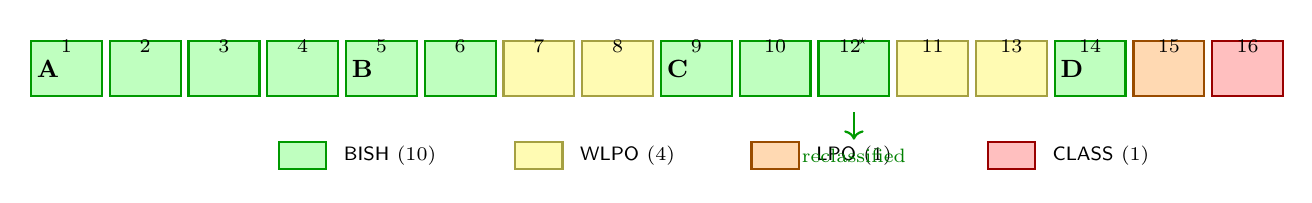
\begin{tikzpicture}[
  bish/.style={fill=green!25, draw=green!60!black, thick},
  wlpo/.style={fill=yellow!30, draw=yellow!60!black, thick},
  lpo/.style={fill=orange!30, draw=orange!60!black, thick},
  class/.style={fill=red!25, draw=red!60!black, thick},
  phase/.style={font=\small\bfseries, anchor=west},
  comp/.style={font=\scriptsize, anchor=south, text=black}
]
% Phase A: 4 BISH
\foreach \i in {0,...,3} {
  \node[bish, minimum width=0.9cm, minimum height=0.7cm] (a\i) at (\i*1.0, 0) {};
}
\node[phase] at (-0.5, 0) {A};
\node[comp] at (0, 0) {\strut 1};
\node[comp] at (1, 0) {\strut 2};
\node[comp] at (2, 0) {\strut 3};
\node[comp] at (3, 0) {\strut 4};

% Phase B: 2 BISH + 2 WLPO
\foreach \i in {4,5} {
  \node[bish, minimum width=0.9cm, minimum height=0.7cm] (b\i) at (\i*1.0, 0) {};
}
\foreach \i in {6,7} {
  \node[wlpo, minimum width=0.9cm, minimum height=0.7cm] (b\i) at (\i*1.0, 0) {};
}
\node[phase] at (3.5, 0) {B};
\node[comp] at (4, 0) {\strut 5};
\node[comp] at (5, 0) {\strut 6};
\node[comp] at (6, 0) {\strut 7};
\node[comp] at (7, 0) {\strut 8};

% Phase C: 3 BISH + 2 WLPO
\foreach \i in {8,9,10} {
  \node[bish, minimum width=0.9cm, minimum height=0.7cm] (c\i) at (\i*1.0, 0) {};
}
\foreach \i in {11,12} {
  \node[wlpo, minimum width=0.9cm, minimum height=0.7cm] (c\i) at (\i*1.0, 0) {};
}
\node[phase] at (7.5, 0) {C};
\node[comp] at (8, 0) {\strut 9};
\node[comp] at (9, 0) {\strut 10};
\node[comp] at (10, 0) {\strut 12${}^{\!\star}$};
\node[comp] at (11, 0) {\strut 11};
\node[comp] at (12, 0) {\strut 13};

% Phase D: 1 BISH + 1 LPO + 1 CLASS
\node[bish, minimum width=0.9cm, minimum height=0.7cm] at (13, 0) {};
\node[lpo, minimum width=0.9cm, minimum height=0.7cm] at (14, 0) {};
\node[class, minimum width=0.9cm, minimum height=0.7cm] at (15, 0) {};
\node[phase] at (12.5, 0) {D};
\node[comp] at (13, 0) {\strut 14};
\node[comp] at (14, 0) {\strut 15};
\node[comp] at (15, 0) {\strut 16};

% Legend
\node[bish, minimum width=0.6cm, minimum height=0.35cm] at (3, -1.1) {};
\node[font=\scriptsize, anchor=west] at (3.4, -1.1) {\BISH{} (10)};
\node[wlpo, minimum width=0.6cm, minimum height=0.35cm] at (6, -1.1) {};
\node[font=\scriptsize, anchor=west] at (6.4, -1.1) {\WLPO{} (4)};
\node[lpo, minimum width=0.6cm, minimum height=0.35cm] at (9, -1.1) {};
\node[font=\scriptsize, anchor=west] at (9.4, -1.1) {\LPO{} (1)};
\node[class, minimum width=0.6cm, minimum height=0.35cm] at (12, -1.1) {};
\node[font=\scriptsize, anchor=west] at (12.4, -1.1) {\CLASS{} (1)};

% Annotation for Component 12
\draw[->, thick, green!60!black] (10, -0.55) -- (10, -0.9);
\node[font=\scriptsize, anchor=north, text=green!50!black] at (10, -0.9) {reclassified};
\end{tikzpicture}
\caption{CRM decomposition of the regular holonomic RH correspondence into 16 components across four phases (A--D).
Component~12${}^{\star}$ is the key reclassification: connection coefficients descend from na\"ive \CLASS{} to \BISH{} via constructive $\Gamma$-evaluation.
The sole \LPO{} obstruction (Component~15, Deligne's canonical extension) and the sole \CLASS{} obstruction (Component~16, GAGA descent) are in Phase~D.}
\label{fig:decomposition}
\end{figure}

\begin{figure}[ht]
\centering
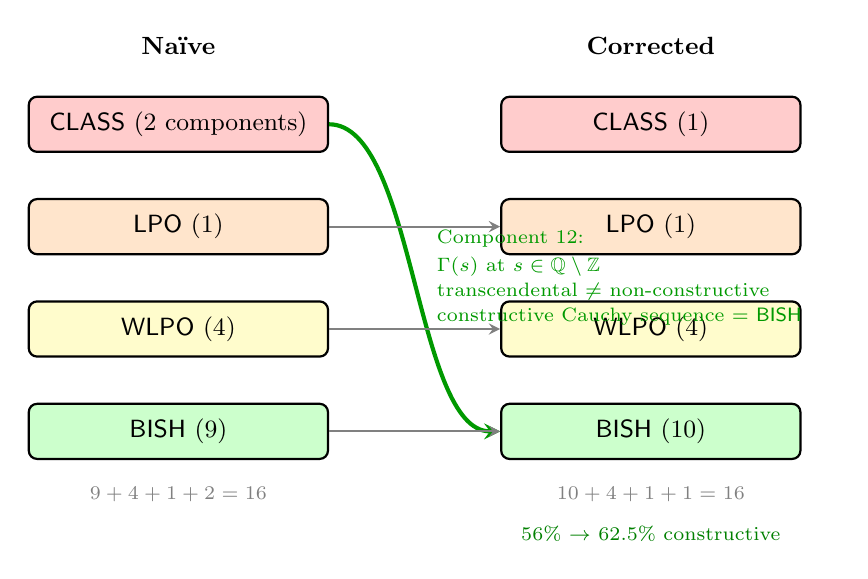
\begin{tikzpicture}[
  level/.style={draw, thick, rounded corners=3pt, minimum width=3.8cm, minimum height=0.7cm, font=\small},
  arrow/.style={->, thick, >=stealth},
  note/.style={font=\scriptsize, text width=5cm, align=left}
]
% Left column: Naive classification
\node[font=\small\bfseries] at (-3, 3.5) {Na\"ive};
\node[level, fill=red!20] (naive-class) at (-3, 2.5) {\CLASS{} (2 components)};
\node[level, fill=orange!20] (naive-lpo) at (-3, 1.2) {\LPO{} (1)};
\node[level, fill=yellow!20] (naive-wlpo) at (-3, -0.1) {\WLPO{} (4)};
\node[level, fill=green!20] (naive-bish) at (-3, -1.4) {\BISH{} (9)};

% Right column: Corrected classification
\node[font=\small\bfseries] at (3, 3.5) {Corrected};
\node[level, fill=red!20] (sq-class) at (3, 2.5) {\CLASS{} (1)};
\node[level, fill=orange!20] (sq-lpo) at (3, 1.2) {\LPO{} (1)};
\node[level, fill=yellow!20] (sq-wlpo) at (3, -0.1) {\WLPO{} (4)};
\node[level, fill=green!20] (sq-bish) at (3, -1.4) {\BISH{} (10)};

% The reclassification arrow
\draw[arrow, green!60!black, line width=1.5pt]
  (naive-class.east) .. controls (0, 2.5) and (0, -1.4) .. (sq-bish.west)
  node[midway, right=4pt, note] {Component 12:\\[2pt]
    $\Gamma(s)$ at $s \in \Q \setminus \Z$\\[1pt]
    transcendental $\neq$ non-constructive\\[1pt]
    constructive Cauchy sequence $=$ \BISH};

% Static arrows
\draw[arrow, gray] (naive-lpo.east) -- (sq-lpo.west);
\draw[arrow, gray] (naive-wlpo.east) -- (sq-wlpo.west);
\draw[arrow, gray] (naive-bish.east) -- (sq-bish.west);

% Tally labels
\node[font=\scriptsize, text=gray] at (-3, -2.2) {$9+4+1+2 = 16$};
\node[font=\scriptsize, text=gray] at (3, -2.2) {$10+4+1+1 = 16$};
\node[font=\scriptsize, text=green!50!black] at (3, -2.7) {56\% $\to$ 62.5\% constructive};
\end{tikzpicture}
\caption{Reclassification of Component~12 (Kummer connection coefficients) from na\"ive \CLASS{} to \BISH.
The na\"ive classification assigns \CLASS{} because $\Gamma$ is transcendental.
The corrected classification recognizes that transcendental $\neq$ non-constructive: $\Gamma(s)$ at non-integral rationals admits constructive Cauchy sequences with explicit moduli of convergence.
No classical proof path is replaced; the descent corrects a misattribution.}
\label{fig:reclassification}
\end{figure}

% ============================================================
\section{Formal Verification}
% ============================================================

The Lean~4 bundle consists of three files totaling 404 lines with 0~\texttt{sorry}, building against Mathlib v4.29.0-rc2:

\begin{center}
\begin{tabular}{lrl}
\toprule
File & Lines & Content \\
\midrule
\texttt{CRMLevel.lean} & 75 & CRM hierarchy, join, ordering \\
\texttt{RHData.lean} & 120 & CAS-emitted: parameters, indicial roots, Fuchs, Deligne \\
\texttt{Paper106\_RiemannHilbert.lean} & 209 & Decomposition, Theorems A--C, test case \\
\bottomrule
\end{tabular}
\end{center}

\subsection{Non-resonance (\BISH): human-readable proof}

The key \BISH{} verification is non-resonance: exponent differences are non-integral.
We prove $1/3 \notin \Z$ by contradiction.

\begin{proof}[Proof of non-resonance at $z = 0$]
Suppose $1/3 = n$ for some $n \in \Z$.
Then $3n = 1$ in $\Z$.
But $3 \mid 3n$ and $3 \nmid 1$, contradiction.
The same argument with denominator~12 handles $z = 1$ and $z = \infty$.
\end{proof}

\noindent
In Lean~4, this is:

\begin{tcolorbox}[leanbox={Non-resonance at z=0 -- RHData.lean}]
\begin{lstlisting}[style=leanstyle]
theorem diff_zero_not_int :
    forall n : Int, diff_zero (*@$\neq$@*) (n : Rat) := by
  intro n; simp only [diff_zero]; intro h
  have : (3 : Rat) * (n : Rat) = 1 := by linarith
  have : (3 : Int) * n = 1 := by exact_mod_cast this
  omega
\end{lstlisting}
\end{tcolorbox}

The tactic chain makes the logical structure transparent: \texttt{linarith} clears the rational arithmetic, \texttt{exact\_mod\_cast} lifts from $\Q$ to $\Z$, and \texttt{omega} discharges $3n = 1$ over $\Z$ by divisibility.
No classical logic enters: $\Q$ arithmetic is decidable by definition (\BISH).

\subsection{Fuchs relation (\BISH): code and proof}

\begin{proof}[Proof of the Fuchs relation]
The six exponents are $0, 1/3, 0, 1/12, 1/4, 1/3$.
Their sum is $0 + 4/12 + 0 + 1/12 + 3/12 + 4/12 = 12/12 = 1$.
For an order-$n$ Fuchsian ODE with $k$ regular singularities on $\PP^1$, the Fuchs relation requires the sum of all $nk$ exponents to equal $\frac{n(n-1)(k-2)}{2}$.
Here $n = 2$, $k = 3$, giving $\frac{2 \cdot 1 \cdot 1}{2} = 1$.
\end{proof}

\begin{tcolorbox}[leanbox={Fuchs relation (Paper106\_RiemannHilbert.lean)}]
\begin{lstlisting}[style=leanstyle]
theorem test_fuchs :
    (0 : Rat) + 1/3 + 0 + 1/12 + 1/4 + 1/3 = 1 := by
  norm_num
\end{lstlisting}
\end{tcolorbox}

\subsection{Deligne strip verification (\BISH{} for $\Q$-exponents)}

\begin{proof}[Proof that Deligne-shifted exponents lie in $[0,1)$]
For the test case, all exponents are already in $[0,1)$: specifically $0, 1/3, 0, 1/12, 1/4, 1/3 \in [0,1)$.
No integer floor shift is needed.
This is the rational collapse of Theorem~C: when exponents are rational and already in $[0,1)$, the Deligne canonical extension is \BISH.
\end{proof}

\begin{tcolorbox}[leanbox={Deligne strip (Paper106\_RiemannHilbert.lean)}]
\begin{lstlisting}[style=leanstyle]
theorem test_deligne_in_strip :
    (0 (*@$\le$@*) (0:Rat) (*@$\wedge$@*) (0:Rat) < 1) (*@$\wedge$@*)
    (0 (*@$\le$@*) (1/3:Rat) (*@$\wedge$@*) (1/3:Rat) < 1) (*@$\wedge$@*)
    (0 (*@$\le$@*) (1/12:Rat) (*@$\wedge$@*) (1/12:Rat) < 1) (*@$\wedge$@*)
    (0 (*@$\le$@*) (1/4:Rat) (*@$\wedge$@*) (1/4:Rat) < 1) := by
  norm_num
\end{lstlisting}
\end{tcolorbox}

\subsection{The \LPO{} boundary: floor function on $\R$}

\begin{proof}[Proof that $\lfloor \cdot \rfloor : \Q \to \Z$ is \BISH]
The floor function on $\Q$ is computed by integer division: $\lfloor p/q \rfloor = \operatorname{div}(p, q)$ (with appropriate sign convention).
This is a finite arithmetic operation, hence \BISH.
For $\R$, the floor function requires deciding $n \le x < n+1$ for each $n \in \Z$, which requires real-valued comparison, equivalent to \LPO{} (Bridges--Richman \cite{BridgesRichman1987}, Theorem~6.1).
\end{proof}

\begin{tcolorbox}[leanbox={Floor function on Q -- Paper106\_RiemannHilbert.lean}]
\begin{lstlisting}[style=leanstyle]
-- BISH: floor on rationals is decidable
def rat_floor (q : Rat) : Int := Int.floor q

-- BISH: fractional part lies in [0, 1)
theorem rat_frac_in_strip (q : Rat) :
    (0 : Rat) (*@$\le$@*) Int.fract q (*@$\wedge$@*) Int.fract q < 1 :=
  (*@$\langle$@*)Int.fract_nonneg q, Int.fract_lt_one q(*@$\rangle$@*)

-- Documentary: a total floor on (*@$\mathbb{R}$@*) implies LPO
axiom floor_implies_LPO :
  ((*@$\exists$@*) f : Real (*@$\to$@*) Int,
    forall x, (f x : Real) (*@$\le$@*) x (*@$\wedge$@*)
              x < (f x : Real) + 1) (*@$\to$@*)
  LPO_statement
\end{lstlisting}
\end{tcolorbox}

The documentary axiom \texttt{floor\_implies\_LPO} states a non-vacuous conditional: if a total floor function on $\R$ exists, then \LPO{} holds.
Unlike the vacuously true $P \Rightarrow \top$ pattern, this axiom has genuine logical content and is unused in any proof.

\subsection{Kummer connection (BISH --- documentary)}

The Kummer connection matrix entries involve Gamma-function ratios at non-integral rational arguments (including $\Gamma(-1/12)$, reduced to the positive domain via $\Gamma(s) = \Gamma(s{+}1)/s$).
These are transcendental but \BISH-computable: $\Gamma(s)$ for $s \in \Q \setminus \Z$ has constructive majorants and moduli of convergence.
Lean records them as comments because Mathlib does not yet implement symbolic $\Gamma$-evaluation.

\begin{tcolorbox}[leanbox={Kummer connection matrix -- documentary}]
\begin{lstlisting}[style=leanstyle]
-- Kummer Connection Matrix (BISH -- documentary)
-- Entries are Gamma-function ratios at non-integral rationals.
-- Functional eqn reduces negative args to positive domain.
-- Computable but not yet formalizable in Mathlib.

-- C01[0,0] = Gamma(1/12)*Gamma(2/3) /
--            (Gamma(1/3)*Gamma(5/12))
--         ~ 2.7320508076

-- C01[1,1] = Gamma(-1/12)*Gamma(4/3) /
--            (Gamma(7/12)*Gamma(2/3))
--         ~ -5.4641016151

-- det(C01) ~ -4.0000000000 (algebraic!)
\end{lstlisting}
\end{tcolorbox}

The transcendental individual entries contrast with the algebraic determinant $\det(C_{01}) = -4$.
This structural feature --- some algebraic invariants survive the archimedean passage --- is a recurring theme in the CRM series (cf.\ the trace vanishing identities of Papers~84--92, which are polynomial identities verifiable by \texttt{ring} despite arising from transcendental monodromy).

\subsection{Axiom inventory}

\begin{tcolorbox}[leanbox={\texttt{\#print axioms} output}]
\begin{lstlisting}[style=leanstyle]
-- Component counting (axiom-free):
-- total_components : does not depend on any axioms
-- constructive_fraction : does not depend on any axioms

-- Algebraic test case (norm_num on Rat):
-- test_fuchs : propext, Classical.choice, Quot.sound
-- test_deligne_in_strip : propext, Classical.choice,
--                         Quot.sound
-- diff_zero_not_int : propext, Quot.sound

-- Documentary (unused in proofs):
-- floor_implies_LPO
-- gaga_descent_requires_LEM
\end{lstlisting}
\end{tcolorbox}

The component counting theorems use \texttt{decide}, which reduces \texttt{Nat} arithmetic in the kernel without invoking any axioms.
The documentary axioms (\texttt{floor\_implies\_LPO}, \texttt{gaga\_descent\_requires\_LEM}) are unused in any proof term.

\subsection{Classical.choice audit}

The \texttt{\#print axioms} command traverses the proof term's dependency graph, not the module environment: importing \texttt{Mathlib.Tactic} does not ``taint'' theorems that do not use classical definitions.
Pure \texttt{Nat} arithmetic via \texttt{decide} is axiom-free, as witnessed by \texttt{total\_components}.
The \texttt{Classical.choice} in \texttt{test\_fuchs} and \texttt{test\_deligne\_in\_strip} enters through Mathlib's generic algebraic hierarchy: \texttt{norm\_num} invokes lemmas over \texttt{DivisionRing} and \texttt{LinearOrderedField}, whose totalized inverse ($0^{-1} = 0$) is defined via classical choice.
The \texttt{Rat} type itself is 100\% computable and axiom-free.
The mathematical content is constructively valid --- $\Q$~arithmetic is decidable by definition (\BISH) --- but the Lean~4 proof term carries the classical dependency as an implementation artifact.
Constructive stratification is established by proof content, not by the axiom checker output.

% ============================================================
\section{Discussion}
% ============================================================

\subsection{Connection to the Archimedean Obstruction Thesis}

Paper~98 (Theorem~5.1) predicts that in arithmetic geometry, classical logic enters through Betti realization --- passage through the archimedean place $\R/\C$.
The RH correspondence is the prototypical Betti realization functor: it converts algebraic $\mathcal{D}$-modules (de~Rham) into topological constructible sheaves (Betti).

Our decomposition confirms the prediction with a sharper result than initially expected.
The algebraic side (Phase~A) is entirely \BISH.
The local analytic theory (Phase~B) introduces \WLPO{} only at equality-testing on $\C$-valued quantities.
The global theory (Phase~C) is \BISH{} + \WLPO{}: the connection coefficients (Gamma-function ratios) are transcendental but \BISH-computable, since completing a computable Cauchy sequence is the definition of a real number in \BISH.
The sole \CLASS{} component is GAGA descent (Phase~D), where the obstruction is Montel's theorem --- infinite-dimensional sequential compactness, not transcendental evaluation.

\subsection{Comparison with Fargues-Scholze}

Paper~99 established $\CRM(\mathrm{FLT}) = \WKL$ by analyzing modularity lifting through Fargues-Scholze's $p$-adic geometrization.
The regular RH correspondence, by contrast, operates over $\C$ and costs \CLASS.
This phase transition --- $\WKL$ for $p$-adic, \CLASS{} for archimedean --- is the signature of the Archimedean Obstruction Thesis.
Condensed mathematics (Clausen-Scholze) systematically deflates continuous topology to profinite combinatorics ($\WKL$), whereas the archimedean topology of $\C$ resists such deflation.

\subsection{Higher categories, Scholze, and the locus of classical cost}

The regular holonomic RH correspondence is a foundational ingredient in the geometric Langlands program.
Gaitsgory et al.\ \cite{Gaitsgory2024} proved the geometric Langlands conjecture (GLC) using the categorical RH equivalence --- Kashiwara's derived category version, not the ODE-level Deligne correspondence we audited --- as a key structural input.
Our decomposition therefore gives a \emph{lower bound}: $\CRM(\mathrm{GLC}) \ge \CRM(\mathrm{RH}_{\mathrm{reg}}) = \CLASS$.
The \CLASS{} component (GAGA descent via Montel's theorem) propagates upward through any proof that invokes the RH correspondence.

\medskip\noindent\textbf{The $\infty$-categorical machinery is logically inert.}
Gaitsgory's proof builds on Lurie's higher algebra \cite{Lurie2017}: $(\infty,1)$-categories, ind-coherent sheaves, and the spectral decomposition of $\QCoh(\Loc_G)$.
Our audit suggests this machinery does not raise the logical cost.
The equivalence of categories (perverse sheaves $\leftrightarrow$ regular holonomic $\mathcal{D}$-modules) is formally \BISH{} once the objects exist: it is a theorem about functors between well-defined categories.
The \CLASS{} cost enters through \emph{constructing} the analytic objects (GAGA), not through the categorical framework.
Upgrading from 1-categories to $(\infty,1)$-categories does not change this: Kan extension is a universal property (\BISH), colimit and adjunction machinery is finitary, and the homotopical bookkeeping of simplicial sets is combinatorial.
The genuine logical cost enters when abstract functors must evaluate concrete archimedean quantities --- the same obstruction we identified in Phases~C and~D.
We therefore expect that $\CRM(\mathrm{GLC}) = \CLASS$, with the $\infty$-categorical layer contributing zero additional omniscience cost.

\medskip\noindent\textbf{Scholze's avoidance of Lurie explained by CRM.}
Scholze's condensed mathematics \cite{ClausenScholze2022} offers a contrasting foundational strategy that CRM clarifies.
The standard account frames Scholze's divergence from Lurie as motivated by set-theoretic concerns (universes, size issues).
CRM suggests a sharper explanation: Scholze is avoiding the \emph{analytic topology} that carries the classical cost, not the higher categories per se.
Lurie's framework accepts the archimedean topology of $\C$ and works within it; condensed mathematics replaces point-set topology (which forces Montel, Baire, Heine-Borel --- exactly the archimedean obstructions that our audit and the Archimedean Obstruction Thesis identify as the \CLASS{} source) with sheaves on profinite sets, routing around the continuous topology entirely.
This is precisely what CRM predicts should lower logical cost: the problem is not categorical complexity but the passage from algebra to analysis.

Paper~99 showed that the Fargues--Scholze $p$-adic replacement lowers $\CRM(\mathrm{FLT})$ from \CLASS{} to \WKL.
The natural test case is whether a \emph{condensed RH correspondence} --- replacing the analytic topology on $X^{\mathrm{an}}$ with its condensed counterpart (Clausen--Scholze's analytic geometry \cite{ClausenScholze2022}) --- could similarly lower Component~16 from \CLASS{} to \WKL{} or below.
Our audit establishes the baseline: classical RH costs $1\ \CLASS$ (GAGA).
If condensed RH eliminates GAGA dependence, that is a genuine logical saving, and AOT predicts exactly this outcome.
We do not claim this is achievable; we flag it as the sharpest testable prediction at the interface of CRM and modern foundations.

\subsection{Position in the CRM program}

Paper~106 is the eighteenth CRMLint application and the first to audit a \emph{categorical equivalence theorem} rather than a single result.
Within the program arc:

\begin{itemize}[nosep]
\item \textbf{Hodge campaign (Papers~84--94):} CRM audits of Hodge-theoretic results (exotic Weil classes, trace vanishing, Griffiths groups). The CLASS obstruction enters through Betti cohomology --- period integrals on complex manifolds.
\item \textbf{Langlands campaign (Papers~95--99):} CRM audits of modularity and BSD. The CLASS obstruction enters through $L$-function evaluation; Fargues-Scholze deflates to WKL.
\item \textbf{RH correspondence (Paper~106):} The \emph{bridge} between the two campaigns. The RH functor \emph{is} the Betti realization that converts algebraic D-modules (de~Rham, the Hodge side) into constructible sheaves (\'etale/Betti, the Langlands side). Our audit shows the bridge itself costs CLASS, with the sole LPO localizing at Deligne's spectral partition.
\end{itemize}

The ``unique LPO'' finding (Theorem~A) demonstrates CRM's resolving power.
Without CRM, the RH correspondence is simply a ``classical theorem.''
With CRM, we see that 10 of its 16 components are constructive, that the four WLPO components are equality tests on $\C$ (not real trichotomy), that the single LPO obstruction admits rational collapse, and that the sole \CLASS{} component is GAGA descent (Montel's theorem).
This granularity is invisible to standard mathematical practice.

The 62.5\% constructive fraction falls in the expected range for archimedean results: Papers~91 (44\%), 94 (67\%), 95 (71\%).
The Archimedean Obstruction Thesis (Paper~98) predicted this range; Paper~106 confirms it on the prototypical Betti realization functor.

\subsection{The irregular RH correspondence}

The irregular case (D'Agnolo--Kashiwara \cite{DAgnoloKashiwara2016}, Mochizuki \cite{Mochizuki2011}) introduces Stokes phenomena: the connection matrices depend not only on the homotopy class of a path but on its geometric direction.
This introduces an additional constructive obstruction beyond \LPO{}: the Stokes multipliers involve asymptotic limits of oscillatory integrals, which may require analytic comprehension principles beyond the CRM hierarchy.
We leave this analysis to future work.

\subsection{Open problems}

\begin{enumerate}[nosep]
\item Is the \WLPO{} tag on Components 8 and 11 tight, or can the identity theorem for convergent power series with algebraic coefficients be reduced to \BISH?
\item Does the irregular RH correspondence require principles beyond \LPO, or does Stokes filtration regularize the constructive cost?
\item Can the GAGA descent (\CLASS) be replaced by an algebraic analogue (e.g., \'etale cohomological descent) that lowers the cost?
\item \textbf{$\infty$-categorical inertness conjecture:} Does the upgrade from $1$-categorical to $(\infty,1)$-categorical RH introduce any omniscience principle not already present in the classical equivalence?  We conjecture no: the logical cost is concentrated in GAGA, not in the categorical framework.
\item \textbf{Condensed RH prediction:} Can a condensed Riemann-Hilbert correspondence (Clausen--Scholze analytic geometry \cite{ClausenScholze2022}) lower Component~16 from \CLASS{} to \WKL{} or below?  The Archimedean Obstruction Thesis predicts this should be possible.
\end{enumerate}

% ============================================================
\section{Conclusion}
% ============================================================

The regular holonomic Riemann-Hilbert correspondence decomposes into $10\ \BISH + 4\ \WLPO + 1\ \LPO + 1\ \CLASS = 16$ components.
Deligne's canonical extension is the unique \LPO{} obstruction, equivalent to the floor function $\lfloor \cdot \rfloor : \R \to \Z$; for rational parameters it collapses to \BISH, witnessed by ${}_2F_1(\tfrac{1}{4}, \tfrac{1}{3}; \tfrac{2}{3}; z)$.
GAGA descent is the unique \CLASS{} obstruction, localized to Montel's theorem (sequential compactness in Cartan's Theorems~A/B).
The connection coefficients, despite being transcendental Gamma-function ratios, are \BISH-computable --- the classical taint enters through infinite-dimensional topology, not through transcendental evaluation.

Three broader conclusions follow.
First, the $\infty$-categorical machinery used in the geometric Langlands proof (Lurie's higher algebra, ind-coherent sheaves, spectral decomposition) is logically inert: Kan extensions, colimits, and simplicial homotopy theory are \BISH{} scaffolding that contributes zero omniscience cost.
The logical expense of the geometric Langlands conjecture is inherited entirely from the RH correspondence's GAGA component.
Second, Scholze's avoidance of Lurie's framework in condensed mathematics is explained by CRM as routing around the archimedean topology --- the \CLASS{} source identified by the Archimedean Obstruction Thesis --- not as avoiding categorical complexity.
Third, this audit establishes the baseline for a testable prediction: a condensed Riemann-Hilbert correspondence, if it eliminates GAGA dependence, would lower the logical cost from \CLASS{} to \WKL{} or below.

% ============================================================
\section*{Acknowledgments}
% ============================================================

This paper was written with the assistance of AI tools (Claude, Anthropic) for proof architecture and Lean~4 formalization.
The mathematical analysis was conducted by the author.
The Lean~4 formalization builds on the Mathlib library \cite{Mathlib}.
This paper follows the format guide of the Constructive Reverse Mathematics Series (DOI: \href{https://doi.org/10.5281/zenodo.18765700}{10.5281/zenodo.18765700}).

% ============================================================
\begin{thebibliography}{30}

\bibitem{Paper1}
P.~C.~K.~Lee, ``The constructive content of classical mathematics,'' Paper~1 of the Constructive Reverse Mathematics Series, Zenodo, 2025.

\bibitem{BishopBridges1985}
E.~Bishop and D.~Bridges, \textit{Constructive Analysis}, Springer, 1985.

\bibitem{BridgesRichman1987}
D.~Bridges and F.~Richman, \textit{Varieties of Constructive Mathematics}, London Math.\ Soc.\ Lecture Note Ser., vol.~97, Cambridge Univ.\ Press, 1987.

\bibitem{Castro1987}
F.~J.~Castro-Jim\'enez, ``Th\'eor\`eme de division pour les op\'erateurs diff\'erentiels et calcul des multiplicit\'es,'' Th\`ese de troisi\`eme cycle, Univ.\ Paris~VII, 1984.

\bibitem{DAgnoloKashiwara2016}
A.~D'Agnolo and M.~Kashiwara, ``Riemann-Hilbert correspondence for irregular holonomic $\mathcal{D}$-modules,'' \textit{Publ.\ Math.\ IH\'ES} \textbf{123} (2016), 69--197.

\bibitem{Deligne1970}
P.~Deligne, \textit{\'Equations diff\'erentielles \`a points singuliers r\'eguliers}, Lecture Notes in Math., vol.~163, Springer, 1970.

\bibitem{BeukersHeckman1989}
F.~Beukers and G.~Heckman, ``Monodromy for the hypergeometric function ${}_nF_{n-1}$,'' \textit{Invent.\ Math.} \textbf{95} (1989), 325--354.

\bibitem{Kashiwara1984}
M.~Kashiwara, ``The Riemann-Hilbert problem for holonomic systems,'' \textit{Publ.\ RIMS, Kyoto Univ.} \textbf{20} (1984), 319--365.

\bibitem{Katz1970}
N.~M.~Katz, ``Nilpotent connections and the monodromy theorem: applications of a result of Turrittin,'' \textit{Publ.\ Math.\ IH\'ES} \textbf{39} (1970), 175--232.

\bibitem{Mathlib}
The Mathlib Community, ``Mathlib: the Lean~4 mathematical library,'' 2024.

\bibitem{Mebkhout1980}
Z.~Mebkhout, ``Sur le probl\`eme de Hilbert-Riemann,'' \textit{C.\ R.\ Acad.\ Sci.\ Paris} \textbf{290} (1980), 415--417.

\bibitem{Mochizuki2011}
T.~Mochizuki, \textit{Wild Harmonic Bundles and Wild Pure Twistor $\mathcal{D}$-Modules}, Ast\'erisque, vol.~340, Soc.\ Math.\ France, 2011.

\bibitem{Oaku1997}
T.~Oaku, ``Algorithms for $b$-functions, restrictions, and algebraic local cohomology groups of $\mathcal{D}$-modules,'' \textit{Adv.\ Appl.\ Math.} \textbf{19} (1997), 61--105.

\bibitem{Serre1956}
J.-P.~Serre, ``G\'eom\'etrie alg\'ebrique et g\'eom\'etrie analytique,'' \textit{Ann.\ Inst.\ Fourier} \textbf{6} (1956), 1--42.

\bibitem{Paper76}
P.~C.~K.~Lee, ``CRMLint: Automated CRM logical cost analyzer,'' Paper~76 of the CRM Series, Zenodo, DOI: 10.5281/zenodo.18779362.

\bibitem{Paper80}
P.~C.~K.~Lee, ``Algebraic Gauss-Manin via Griffiths pole reduction over $\Q(t)$: A CRMLint squeeze,'' Paper~80 of the CRM Series, Zenodo, DOI: 10.5281/zenodo.18791985.

\bibitem{Paper82}
P.~C.~K.~Lee, ``Picard-Fuchs monodromy via Kovacic's algorithm: A CRMLint squeeze,'' Paper~82 of the CRM Series, Zenodo, DOI: 10.5281/zenodo.18801822.

\bibitem{Paper98}
P.~C.~K.~Lee, ``The motivic CRM architecture: Why the six domains of mathematics have different logical signatures,'' Paper~98 of the CRM Series, Zenodo, DOI: 10.5281/zenodo.18902037.

\bibitem{Paper99}
P.~C.~K.~Lee, ``The Hecke theta series squeeze: Resolving the dihedral base case of modularity via Mumford's algebraic theta functions,'' Paper~99 of the CRM Series, Zenodo, DOI: 10.5281/zenodo.18821004.

\bibitem{Gaitsgory2024}
D.~Gaitsgory et al., ``Proof of the geometric Langlands conjecture,'' preprint, 2024. arXiv:2405.03599.

\bibitem{Lurie2017}
J.~Lurie, \textit{Higher Algebra}, 2017. Available at \url{https://www.math.ias.edu/~lurie/papers/HA.pdf}.

\bibitem{ClausenScholze2022}
D.~Clausen and P.~Scholze, ``Condensed mathematics and complex geometry,'' lecture notes, 2022. Available at \url{https://www.math.uni-bonn.de/people/scholze/Complex.pdf}.

\end{thebibliography}

\end{document}
